\documentclass{beamer}
\usepackage{listings}
\lstset{
%language=C,
frame=single, 
breaklines=true,
columns=fullflexible
}
\usepackage{subcaption}
\usepackage{url}
\usepackage{tikz}
\usepackage{tkz-euclide} % loads  TikZ and tkz-base
%\usetkzobj{all}
\usetikzlibrary{calc,math}
\usepackage{float}
\newcommand\norm[1]{\left\lVert#1\right\rVert}
\renewcommand{\vec}[1]{\mathbf{#1}}
\usepackage[export]{adjustbox}
\usepackage[utf8]{inputenc}
\usepackage{amsmath}
\usetheme{Boadilla}

\usetkzobj{all}

\title{Solution For The School Geometry Problems}
\author{Yogesh Choudhary}
%\institute{Indian Institute of Technology, Bhilai.}
\date{\today}
\begin{document}


\begin{frame}
\titlepage
\end{frame}
\section{Question}
\begin{frame}
\frametitle{Question}
\begin{block}{Exercise 8.1(Q no.36)}
Two sides AB and BC and median AM of one
triangle ABC are respectively equal to sides PQ
and QR and median PN of $\Delta$ PQR.Show that
\newline
\hyperlink{a}{\beamerbutton{a)$\Delta$ ABM $\cong$ $\Delta$ PQN}}
\newline
\hyperlink{b}{\beamerbutton{b)$\Delta$ ABC $\cong$ $\Delta$ PQR}}
\newline

\end{block}
\end{frame}

\section{\textbf{Construction}}
\subsection*{Codesandfigures}
\begin{frame}[fragile]
\frametitle{Codes and Figures}
\tiny
\begin{flushleft}
The python code for the figure is
\begin{lstlisting}
./code/Traingle.py
\end{lstlisting}
The latex- tikz code is
\begin{lstlisting}
./figs/triangle.tex
\end{lstlisting}
The above latex code can be compiled as standalone document
\begin{lstlisting} 
./figs/triangle_fig.tex
\end{lstlisting}
\end{flushleft}.
%\begin{columns}
%\column{0.5\textwidth}
\begin{figure}
\begin{minipage}{0.45\linewidth}
\begin{subfigure}{0.5\textwidth}

\begin{flushleft}

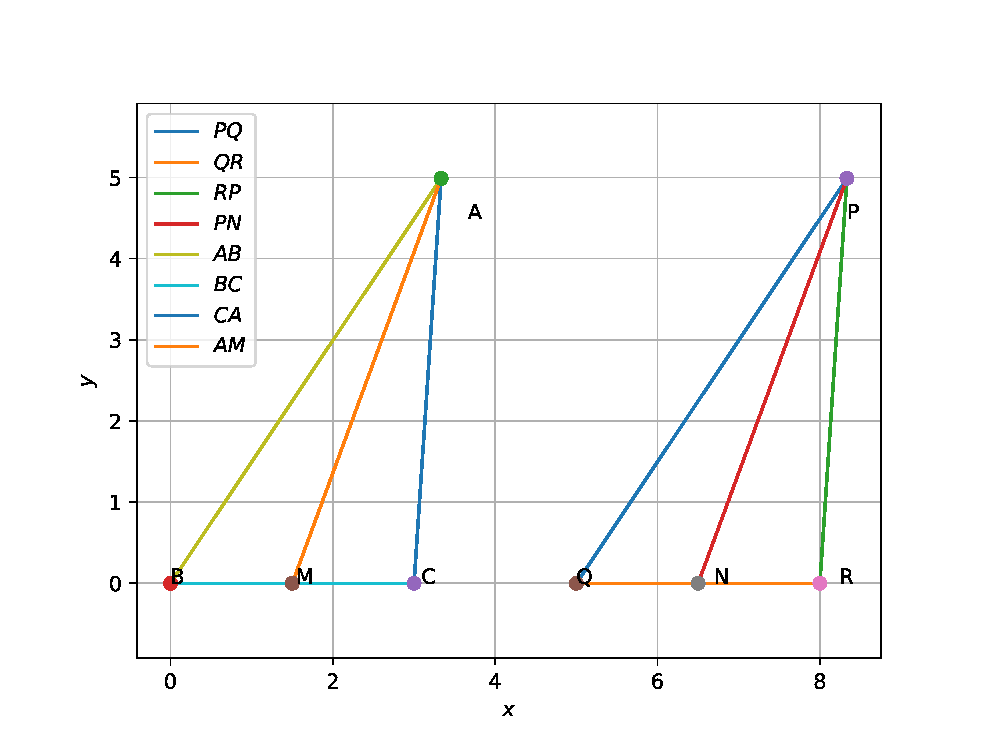
\includegraphics[scale=0.275]{./figs/Triangle.eps}
\caption{\tiny By Python}
\end{flushleft}

\end{subfigure}
\end{minipage}
\hfill
\begin{minipage}{0.45\linewidth}
\begin{subfigure}{0.5\textwidth}
\begin{flushright}

\resizebox{2.0\columnwidth}{!}{

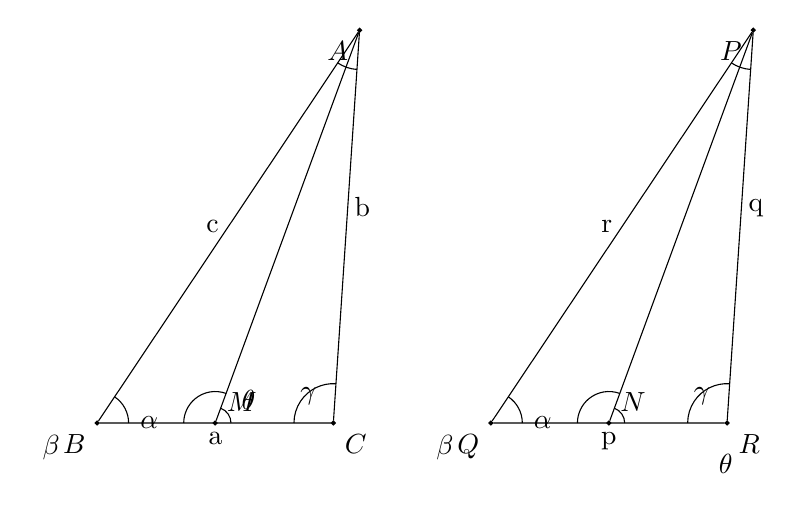
\begin{tikzpicture}
[scale=1,>=stealth,point/.style={draw,circle,fill = black,inner sep=0.5pt},]

\def\a{3}
\def\c{6}
\def\b{5}
\def\x{((\a^2+\c^2-\b^2)/(2*\a))}
\def\y{sqrt(\c^2-\x^2)}


\node (P) at ($({((\a^2+\c^2-\b^2)/(2*\a) +5)},{sqrt(\c^2-\x^2)} )$)[point,label=below left:$P$] {};
\node (Q) at (5, 0)[point,label=below left:$Q$] {};
\node (R) at (\a + 5, 0)[point,label=below right:$R$] {};
\node (N) at ($({(\a/2) +5} , 0)$)[point,label=above right:$N$] {};

\node (A) at ($({((\a^2+\c^2-\b^2)/(2*\a))},{sqrt(\c^2-\x^2)} )$)[point,label=below left:$A$] {};
\node (B) at (0, 0)[point,label=below left:$B$] {};
\node (C) at (\a, 0)[point,label=below right:$C$] {};
\node (M) at ($({\a/2}, 0)$)[point,label=above right:$M$] {};


\draw (P) -- node[left] {$\textrm{r}$} (Q) -- node[below] {$\textrm{p}$} (R) -- node[above,xshift=2mm] {$\textrm{q}$} (P);
\draw (P)--(N);

\draw (A) -- node[left] {$\textrm{c}$} (B) -- node[below] {$\textrm{a}$} (C) -- node[above,xshift=2mm] {$\textrm{b}$} (A);
\draw (A)--(M);

\tkzMarkAngle[fill=orange!40,size=0.5cm,mark=](P,R,Q)
\tkzMarkAngle[fill=orange!40,size=0.4cm,mark=](N,Q,P)
\tkzMarkAngle[fill=green!40,size=0.5cm,mark=](Q,P,R)
\tkzMarkAngle[fill=blue!40,size=0.4cm,mark=](P,N,Q)
\tkzMarkAngle[fill=red!40,size=0.2cm,mark=](R,N,P)
\tkzLabelAngle[pos=0.45](P,R,Q){$\gamma$}
\tkzLabelAngle[pos=0.65](P,Q,R){$\beta$}
\tkzLabelAngle[pos=0.65](R,Q,N){$\alpha$}
\tkzLabelAngle[pos=0.5](R,R,P){$\theta$}

\tkzMarkAngle[fill=orange!40,size=0.5cm,mark=](A,C,B)
\tkzMarkAngle[fill=orange!40,size=0.4cm,mark=](M,B,A)
\tkzMarkAngle[fill=green!40,size=0.5cm,mark=](B,A,C)
\tkzMarkAngle[fill=blue!40,size=0.4cm,mark=](A,M,B)
\tkzMarkAngle[fill=red!40,size=0.2cm,mark=](C,M,A)
\tkzLabelAngle[pos=0.45](A,C,B){$\gamma$}
\tkzLabelAngle[pos=0.65](A,B,C){$\beta$}
\tkzLabelAngle[pos=0.65](C,B,M){$\alpha$}
\tkzLabelAngle[pos=0.5](C,M,A){$\theta$}

\end{tikzpicture}
}
\caption{\tiny By Latex-tikz}
\end{flushright}
\end{subfigure}
\end{minipage}
\end{figure}
\end{frame}
\subsection*{Construction methods}
\begin{frame}[fragile]
\footnotesize
\frametitle{Construction method}
\begin{columns}
\begin{column}{0.5\textwidth}
The tables below are the values used for constructing the triangles in both Python and Latex-Tikz.
\begin{table}[htbp]
\centering
  \resizebox{0.75\textwidth}{!}{\begin{minipage}{\textwidth}
\begin{tabular}{ |p{3cm}|p{3cm}|  }
\hline
 \multicolumn{2}{|c|}{Initial Input Values.} \\
\hline
a, p & 3\\
\hline
b, q & 5\\
\hline
c, r & 6\\
\hline
\end{tabular}
\end{minipage}}
\caption{\tiny To construct $\triangle ACB$ and $\triangle PQR$}
\end{table}
The steps for constructing $\triangle ACB$ are
\newline
$$(i)\vec{A}= \begin{pmatrix}3.33\\4.99\end{pmatrix}
(ii)\vec{B}=\begin{pmatrix}0\\0\end{pmatrix}
(iii)\vec{C}=\begin{pmatrix}3\\0\end{pmatrix}$$
\\
$$(i)\vec{P}= \begin{pmatrix}8.33\\4.99\end{pmatrix}
(ii)\vec{Q}=\begin{pmatrix}5\\5\end{pmatrix}
(iii)\vec{R}=\begin{pmatrix}8\\0\end{pmatrix}$$
\end{column}
\begin{column}{0.5\textwidth}
$\vec{M}$ and $\vec{N}$ are the midpoints of BC and QR respectively 
\\
$$\vec{M}=\begin{pmatrix}1.5\\0\end{pmatrix},\vec{N}=\begin{pmatrix}6.5\\0\end{pmatrix}$$
\\

\begin{table}[H]
\centering
\resizebox{0.75\textwidth}{!}{\begin{minipage}{\textwidth}
\begin{tabular}{ |p{2cm}|p{2cm}|  }
\hline
 \multicolumn{2}{|c|}{Derived Values for $triangle DCB$.} \\
\hline
$\vec{M}$ & $$\begin{pmatrix}1.5\\0\end{pmatrix}$$\\				
\hline
$\vec{N}$ & $$\begin{pmatrix}6.5\\0\end{pmatrix} $$\\
\hline
\end{tabular}
\end{minipage}}
\caption{\tiny To construct madians AN and PN}
\end{table}
\end{column}
\end{columns}
\end{frame}
\section*{\textbf{Solution}}
\begin{frame}[fragile]
\footnotesize
\frametitle{Solution}
\begin{columns}
\begin{column}{0.5\textwidth}
given that $\to$
\\
$$AB = PQ=c=r$$ 
\\

$$BC=QR=a=p$$ 
\\

$$AM=PN=m=n$$ 

\end{column}
\begin{column}{0.5\textwidth}
Therefore $\to$
\\

$\vec{M}$  and $\vec{N}$ are the position vector of mid-point of $\vec{BC}$ and $\vec{QR}$ repectively .
\newline
$$\frac{1}{2}BC= \frac{1}{2}QR$$
\\
\end{column}
\end{columns}
\end{frame}
\subsection{a}
\begin{frame}
\frametitle{Solution a)}
\footnotesize
\label{a}
from triangles ABM and PQR $\to$
\\
$$AB=PQ(given)$$
\\
$$AM=PN(given)$$
\\
$$MB =NQ$$(Both m and N are the mid points)
\newline
\\
$\implies \triangle ABM$ and $\triangle PQN$ are congruent to each other by SSS congruency.
\\
Hence, proved
\end{frame}

\subsection{a}
\begin{frame}
	\frametitle{Solution b)}
	\footnotesize
	\label{b}
		given that $\to$
	\\
	$$MC = NR$$ 
	\\
	$$\because \Delta ABM \cong \Delta PQN $$
	\\
	$$\implies \angle AMC = \angle PNR$$
	
	from SAS congurancy $ \to$
	\\
	$$\Delta AMC \cong \Delta PNR$$
	\\
	$$\implies AC = PR$$
	\\
	Thus from the triangle ABC ,PQR and by SSS congurancy 
	$$\Delta ABC \cong \Delta PQR$$
	\centering Hence proved
\end{frame}

\end{document}
